\section{Pianificazione}
La fase di pianificazione consiste nella suddivisione del lavoro tra i vari componenti del gruppo \Gruppo . La suddivisione deve essere equa e deve fare in modo che ogni componente abbia la possibilità di ricoprire almeno una volta tutti i ruoli. Sono stati determinati cinque periodi principali per suddividere il lavoro:
\begin{itemize}
\item analisi;
\item consolidamento dei \glo{requisiti};
\item progettazione architetturale;
\item progettazione di dettaglio e codifica;
\item \glo{validazione} e collaudo.
\end{itemize}
Ognuno di questi viene poi suddiviso in diversi \glo{sprint} dove vengono individuate le attività che verranno realizzate.
Infine, ogni periodo viene riassunto nel corrispettivo \glo{diagramma di Gantt} e rappresentato tramite \glo{timeline} delle quali viene riportata la legenda dei colori in seguito.

\subsubsection{Legenda dei colori delle timeline}
\begin{figure}[H]
	\centering
    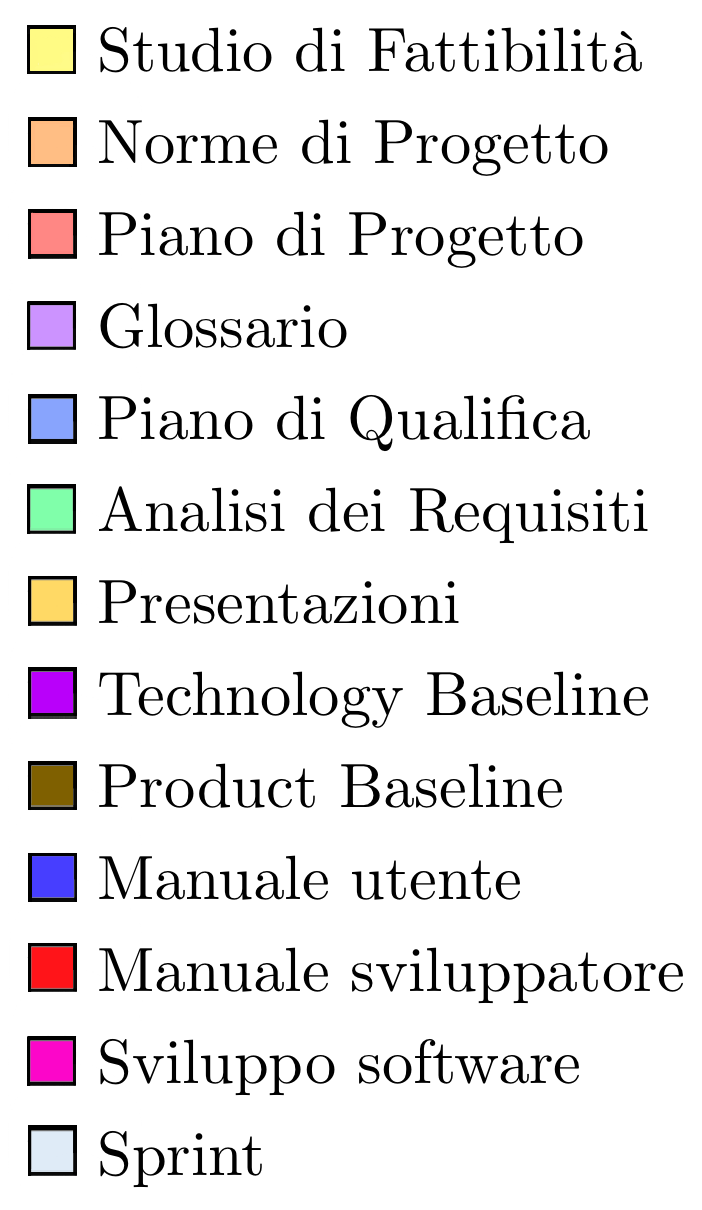
\includegraphics[scale = 0.5]{components/img/legenda.png}
    \caption{Legenda dei colori delle timeline}
    \label{fig:Legenda dei colori delle timeline}
\end{figure}

\subsection{Analisi}
Questo periodo ha inizio il 2020-11-09 procede con quattro fasi fino al 2021-01-11.
Durante il suo decorso i ruoli attivi sono:
\begin{itemize}
\item \textit{responsabile};
\item \textit{amministratore};
\item \textit{analista};
\item \textit{verificatore}.
\end{itemize}
Le precondizioni sono:
\begin{itemize}
	\item formazione del gruppo;
	\item presentazione dei capitolati.
\end{itemize}
Le post condizioni sono:
\begin{itemize}
	\item scelta del nome e del logo del gruppo;
	\item creazione della e-mail;
	\item scelta del capitolato su cui svolgere il progetto;
	\item redazione dei documenti quali: \SdF{}, \NdP{}, \PdP{}, \G{}, \LdP{}, \PdQ{}, \AdR{} e i verbali;
	\item \glo{verifica} e approvazione dei documenti.
\end{itemize}
\subsubsection{Attività}
Questo periodo è composto da sette attività che corrispondono alla produzione dei seguenti documenti:
\begin{itemize}
	\item \textbf{Studio di Fattibilità:} viene fatta una discussione su ogni capitolato, rilevandone pro e contro di ognuno di essi, e dopo un periodo di studio e analisi il gruppo pone la sua preferenza in uno dei capitolati proposti;
	\item \textbf{Norme di Progetto:} vengono definite tutte le regole che il gruppo dovrà rispettare durante lo sviluppo del progetto, tra cui norme relative al prodotto da realizzare e ai processi da adottare;
	\item \textbf{Individuazione degli strumenti:} consiste nel determinare quali strumenti devono essere utilizzati dal gruppo; vengono ricercati strumenti per la comunicazione, per la stesura dei documenti, per lo sviluppo e la \glo{verifica} del \glo{software};
	\item \textbf{Analisi dei \ignore{Requisiti}:} viene analizzato il capitolato scelto nell'attività di \SdF{} e vengono identificanti i \glo{requisiti} del capitolato; il documento viene composto dagli \textit{analisti};
	\item \textbf{Piano di Progetto:} attività di pianificazione dei compiti e suddivisione dei ruoli dove viene calcolato il preventivo per la realizzazione di progetto; il documento viene composto dal \textit{responsabile};
	\item \textbf{Piano di Qualifica:} si individuano i metodi necessari per garantire la qualità del prodotto; viene redatto dall'\textit{amministratore} e dal \textit{progettista};
	\item\textbf{Glossario:} si individuano tutti i termini che possono risultare ambigui e vengono affiancati da una definizione all'interno del documento;  
	\item \textbf{Lettera di Presentazione:} documento in cui il gruppo \Gruppo{} si candida come fornitore del prodotto \glo{software} richiesto.
\end{itemize}
\subsubsection{Sprint}
La pianificazione di questo periodo è stata suddivisa nei seguenti \glo{sprint}:
\begin{itemize}
	\item \textbf{\ignore{Sprint} 1, dal 2020-11-24 al 2020-12-07:}
	\begin{itemize}
	\item vengono prese decisioni riguardanti: il nome del \glo{team}, l'indirizzo e-mail, il logo, la frequenza degli incontri e gli strumenti per la comunicazione;
	\item viene svolta la discussione sui capitolati, esponendo le preferenze personali dei membri del gruppo. Viene, quindi, svolta l'analisi dei capitolati dove, per ognuno di essi, vengono esaminati pro e contro e vengono effettuate delle valutazioni sui rischi. Successivamente può iniziare la stesura dello Studio di Fattibilità;
	\item viene iniziata la stesura delle \NdP{} per fissare le regole delle attività del gruppo;
	\item inizio della stesura del \PdP{}, dove viene descritta la pianificazione del lavoro da svolgere e la suddivisione dei ruoli tra i membri del gruppo;
	\item vengono stesi i verbali interni relativi alle riunioni del gruppo.
	\end{itemize}
	\item \textbf{\ignore{Sprint} 2, dal 2020-12-08 al 2020-12-22:}
	\begin{itemize}
		\item viene conclusa la stesura delle \NdP{};
		\item viene conclusa la stesura del \PdP{}, eccetto il consuntivo;
		\item inizio stesura del \textit{Glossario}, registrando i termini usati nei documenti che risultano ambigui;
		\item vengono stesi i verbali interni relativi agli incontri svolti durante questo \glo{sprint}.
	\end{itemize}
	\item \textbf{\ignore{Sprint} 3, dal 2020-12-23 al 2021-01-04:}
	\begin{itemize}
		\item il gruppo inizia ad analizzare il capitolato scelto, ricercando i \glo{requisiti} e procedendo con la stesura dell'\AdR{};
		\item si procede con la stesura del \PdQ{}, individuando i metodi per garantire la qualità del prodotto;
		\item stesura della \textit{Lettera di Presentazione};
		\item vengono stesi i verbali interni relativi agli incontri svolti durante questo \glo{sprint}.
	\end{itemize}
	\item \textbf{\ignore{Sprint} 4, dal 2021-01-05 al 2021-01-11 :}
	\begin{itemize}
		\item viene completata la stesura del \textit{Glossario};
		\item viene completata la stesura del \AdR{};
		\item il gruppo uniforma tutti i documenti prodotti alle regole stabilite nelle \NdP{} se necessario;
		\item viene steso il consuntivo finale riguardante il periodo effettuato;
		\item vengono svolte le ultime attività di \glo{verifica} sui documenti.
	\end{itemize}
\end{itemize}

\subsubsection{Diagramma di Gantt: analisi}
\begin{figure}[H]
    \centering
    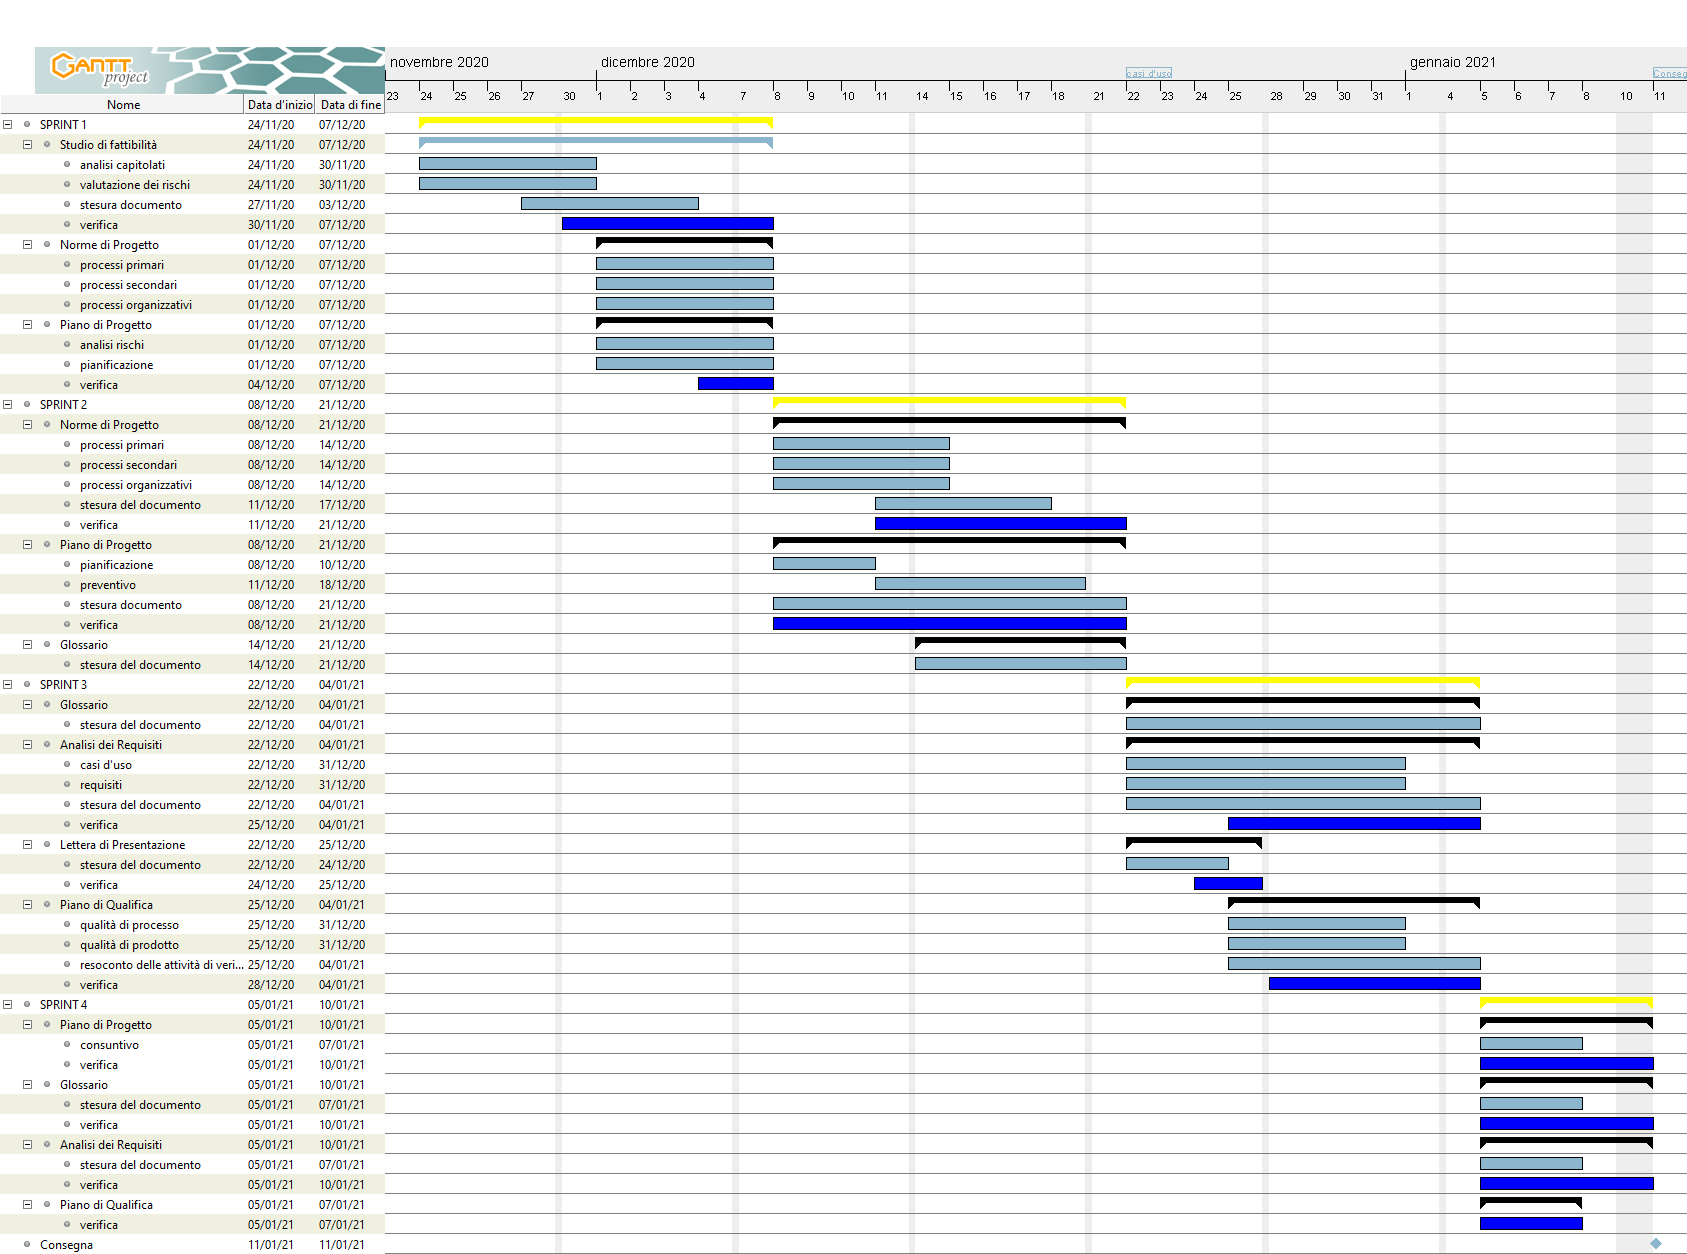
\includegraphics[scale = 0.25]{components/img/Analisi.png}
    \caption{Diagramma di Gantt della fase di Analisi}
    \label{fig:Diagramma di Gantt,  fase di analisi}
\end{figure}
\newpage
\subsection{Consolidamento dei requisiti}
Questo periodo ha inizio il 2021-01-12 e si conclude il 2021-01-18.
le precondizioni sono:
\begin{itemize}
	\item le post condizioni della fase precedente;
	\item consegna dei documenti richiesti.
\end{itemize}
Le post condizioni sono:
\begin{itemize}
	\item conclusione della preparazione della presentazione da esporre per la Revisione dei \ignore{Requisiti};
	\item i componenti devono essere preparati per l'utilizzo delle tecnologie necessarie.
\end{itemize}
\subsubsection{Attività}
Le attività che vengono svolte sono:
\begin{itemize}
	\item miglioramento dei documenti e \glo{verifica};
	\item preparazione alla presentazione per la Revisione dei \ignore{Requisiti};
	\item studio autonomo che ogni componente dovrà effettuare per approfondire le tecnologie necessarie nelle prossime fasi.
\end{itemize}
\subsubsection{Diagramma di Gantt, fase di consolidamento dei requisiti}
\begin{figure}[H]
    \centering
    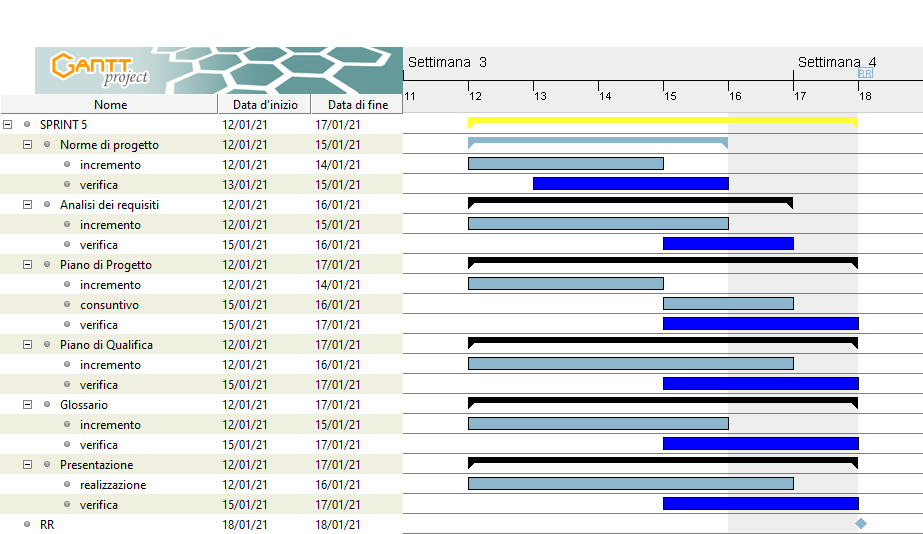
\includegraphics[scale = 0.4]{components/img/consolidamento_requisiti.png}
    \caption{Diagramma di Gantt della fase di Consolidamento dei Requisiti}
    \label{fig:Diagramma di Gantt, fase di consolidamento dei requisiti}
\end{figure}

\newpage
\subsection{Progettazione architetturale}
Questo periodo ha inizio il 2021-01-19 e si conclude il 2021-03-10.
Le precondizioni sono:
\begin{itemize}
	\item le post condizioni del periodo precedente;
	\item è stata approvata la candidatura del gruppo al capitolato \textit{C7}.
\end{itemize}
Le post condizioni sono:
\begin{itemize}
	\item correzione ed incremento dei documenti documenti già prodotti;
	\item produzione del \glo{Proof of Concept};
	\item completamento della progettazione ad alto livello del \glo{software};
	\item consegna dei documenti richiesti alla Revisione di Progettazione; 	
	\item conclusa la preparazione della presentazione da esporre in sede di revisione.
\end{itemize}
\subsubsection{Attività}
Le attività da svolgere durante il periodo sono:
\begin{itemize}
	\item \textbf{Analisi modifiche e \ignore{verifica}:} i documenti già prodotti vengono migliorati e aggiornati se necessario (\NdP{}, \PdP{}, \G{}, \PdQ{}, \AdR{});
	\item \textbf{Technology Baseline:} viene fatta un'analisi ad alto livello del \glo{software} e vengono individuati i design pattern che verranno adottati per lo sviluppo. Infine, viene codificato il \glo{Proof of Concept}, il quale viene presentato o condiviso al committente e al \glo{proponente} in data 2021-03-05.
\end{itemize}
\subsubsection{Timeline: sprint 6 e 7}
\begin{figure}[H]
    \centering
    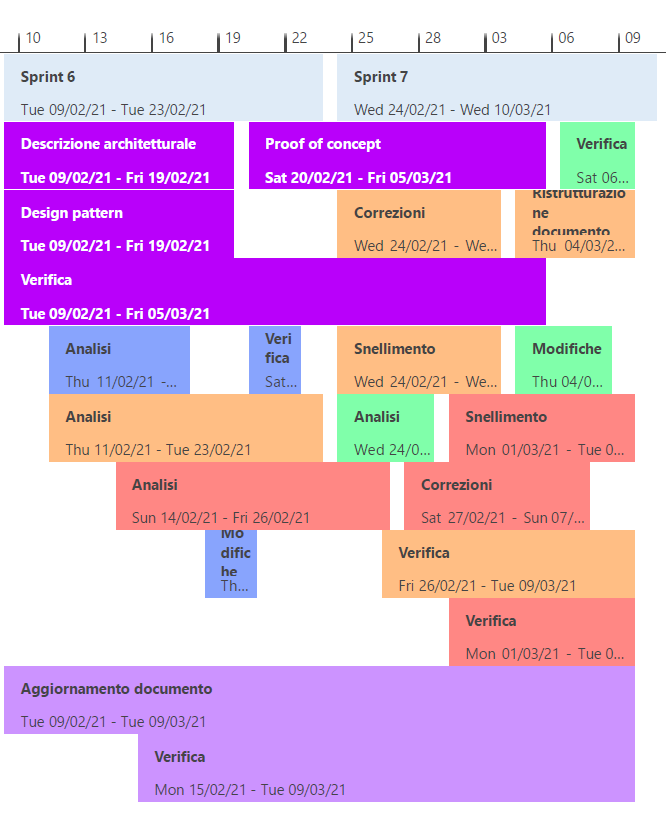
\includegraphics[scale = 0.5]{components/img/sprint6-7.png}
    \caption{Timeline degli sprint che comprendono la  fase di progettazione architetturale}
    \label{fig:Timeline,sprint 6 e 7, fase di progettazione architetturale}
\end{figure}

\subsubsection{Diagramma di Gantt, progettazione architetturale}
\begin{figure}[H]
    \centering
    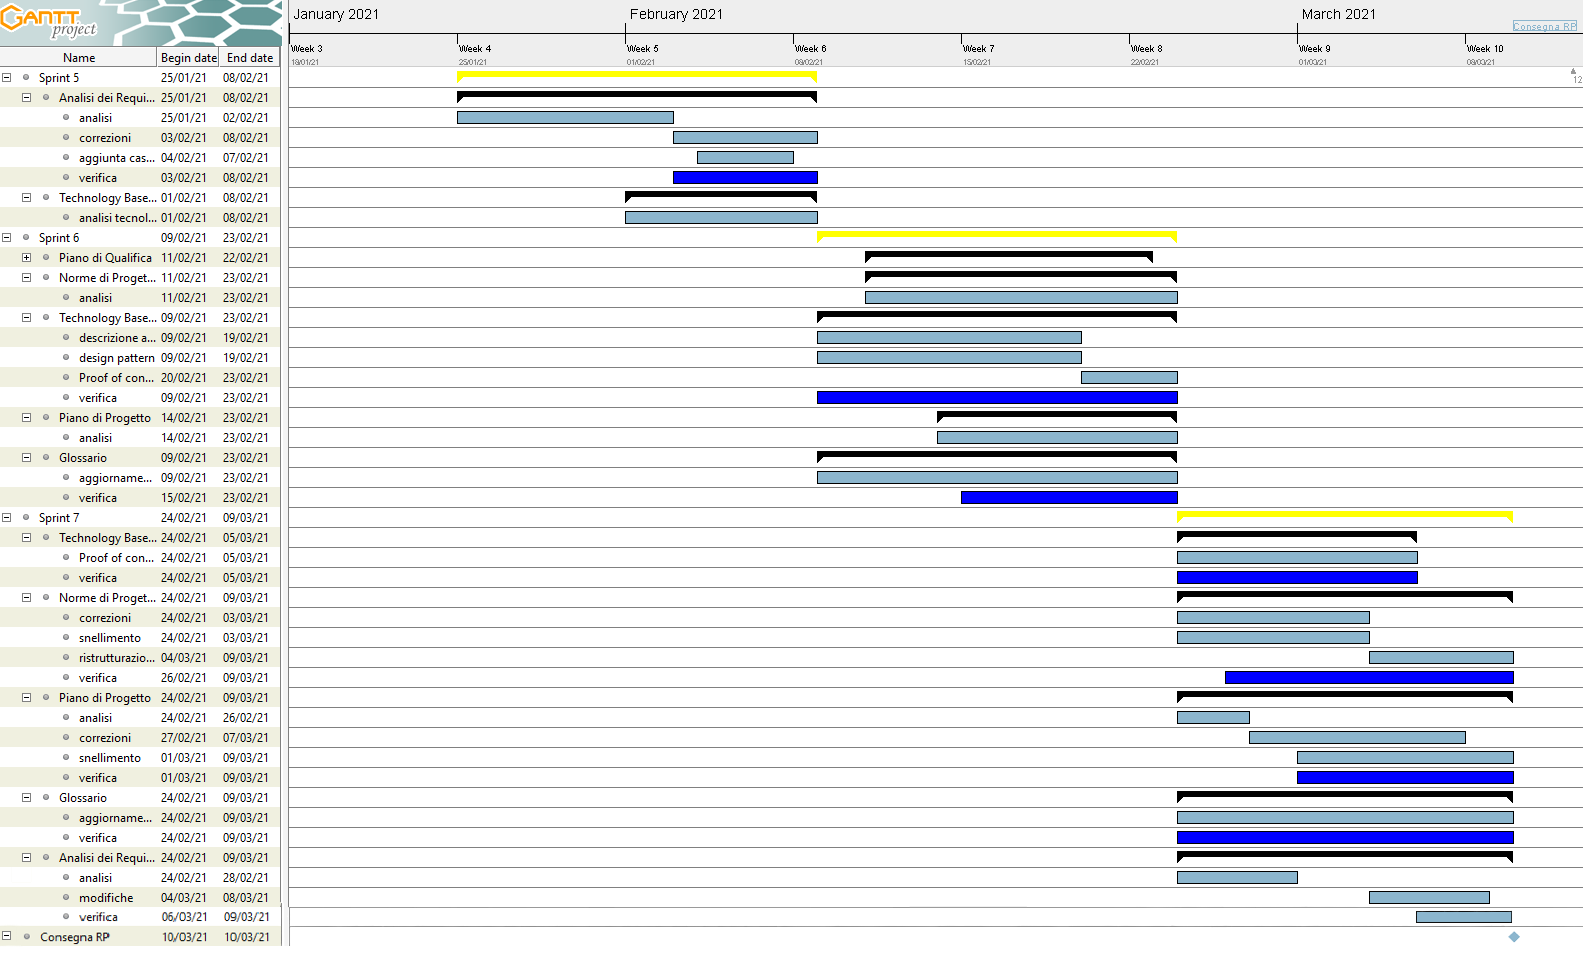
\includegraphics[scale = 0.8]{components/img/progettazione_architetturale.png}
    \caption{Diagramma di Gantt della fase di Progettazione Architetturale}
    \label{fig:Diagramma di Gantt, fase di progettazione architetturale}
\end{figure}

\newpage
\subsection{Progettazione di dettaglio e codifica}
Questo periodo ha inizio il 2021-03-11 e si conclude il 2021-04-09, include lo sprint 8 e lo sprint 9.
Le precondizioni sono:
\begin{itemize}
	\item aggiornamento e correzione dei documenti;
	\item definizione dell'architettura ad alto livello per il \glo{software};
	\item  superamento del colloquio per la \textit{Technology Baseline}.
\end{itemize}
Le post condizioni sono:
\begin{itemize}
	\item aggiornamento e correzione dei documenti;
	\item stesura del \textit{Manuale Utente};
	\item stesura del \textit{Manuale Sviluppatore};
	\item superamento del colloquio per la \textit{Product Baseline};
	\item completamento della codifica e della relativa \glo{verifica} del prodotto \glo{software}.
\end{itemize}
\subsubsection{Attività}
Le attività che vengono svolte sono:
\begin{itemize}
	\item \textbf{Analisi modifiche e \ignore{verifica}:} vengono aggiornati e migliorati i documenti(\NdP{}, \PdP{}, \G{}, \PdQ{}, \textit{Technology Baseline});
	\item \textbf{Product Baseline:} segue la \textit{Technology Baseline}, vengono analizzate più in dettaglio le \glo{unità} i design pattern, le classi e le attività necessarie alla codifica;
	\item \textbf{Sviluppo \ignore{software}:} questa attività consiste nella scrittura dei \glo{test}, nella scrittura del codice e della sua \glo{verifica};
	\item \textbf{Manuale Utente:} viene redatto un documento che descrive tutte le istruzioni d'uso per l'utente;
	\item \textbf{Manuale Sviluppatore:} consiste nella stesura del \textit{Manuale Sviluppatore}.
\end{itemize}
\subsubsection{Diagramma di Gantt, progettazione di dettaglio e codifica}
\begin{figure}[H]
    \centering
    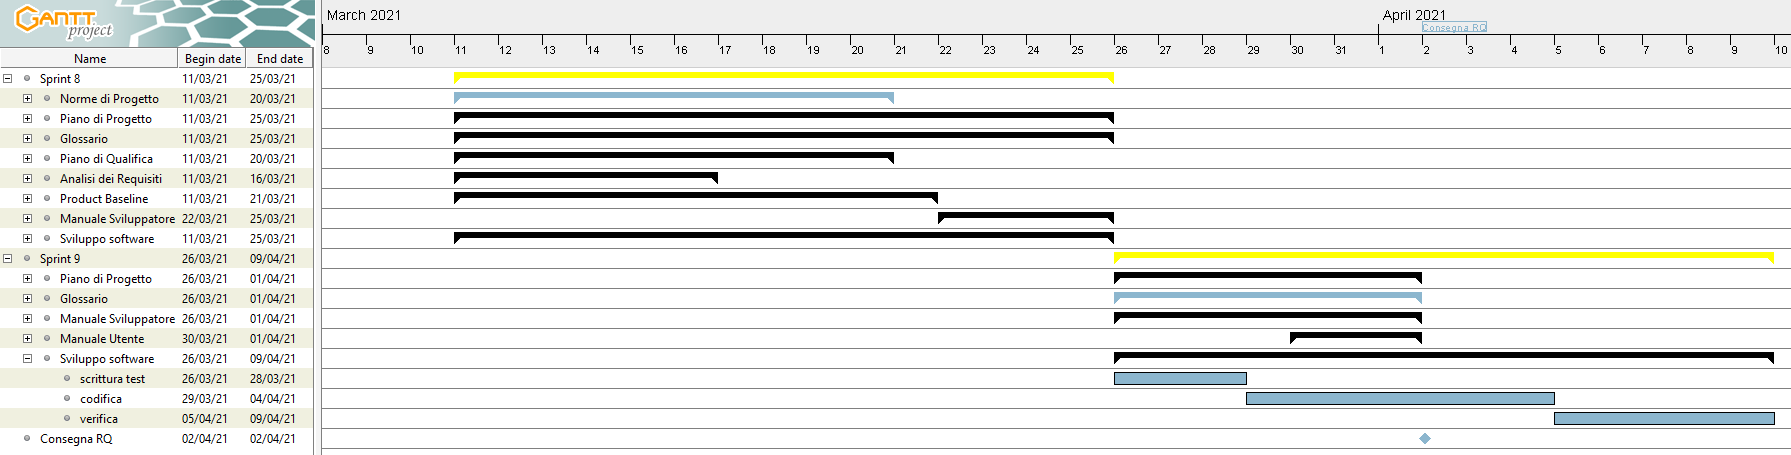
\includegraphics[scale = 0.33]{components/img/progettazione_dettaglio_codifica.png}
    \caption{Diagramma di Gantt della fase di Progettazione di Dettaglio e Codifica}
    \label{fig:Diagramma di Gantt, fase di progettazione di dettaglio e codifica}
\end{figure}
\subsubsection{Sprint 8}
Questo sprint ha inizio in data 2021-03-11 e si conclude in data 2021-03-25.  Le sue precondizioni sono il raggiungimento degli obiettivi dello sprint precedente.\newline{}
Gli obiettivi da raggiungere durante questo periodo sono:
\begin{itemize}
	\item Correzione e verifica delle \NdP{};
	\item Aggiornamento, correzione e verifica del \PdP{};
	\item Redazione introduzione, informazioni su tecnologie, librerie e setup dell'ide nel documento del \MS{};
	\item Aggiornamento, correzione e verifica del \PdQ{};
	\item Correzione UC1, UC2, UC3, UC4 ed UC6 del \AdR{};
	\item Studio design pattern;
	\item Realizzazione diagrammi dei pacchetti, di classe e di sequenza;
	\item Stesura test;
	\item Implementazione pattern scelti;
	\item Implementazione gestione errori di rete;
	\item Verifica del codice;
	\item Aggiornamento del \G{}.
\end{itemize}

\subsubsection{Sprint 9}
Questo sprint ha inizio in data 2021-03-26 e si conclude in data 2021-04-09. Le sue precondizioni sono il raggiungimento degli obiettivi dello sprint precedente.\newline{}
Gli obiettivi da raggiungere durante questo periodo sono:
\begin{itemize}
	\item Redazione test ed architettura nel documento \MS{}
	\item Verifica del \MS{}
	\item Aggiornamento, correzione e verifica del \PdP{};
	\item Realizzazione e verifica del \MU{}
	\item Stesura test;
	\item Rifattorizzazione algoritmo di sincronizzazione;
	\item Miglioramento GUI;
	\item Pulizia del codice;
	\item Aggiornamento e verifica del \G{}.
\end{itemize}
\subsubsection{Timeline: sprint 8 e 9}

\begin{figure}[H]
    \centering
    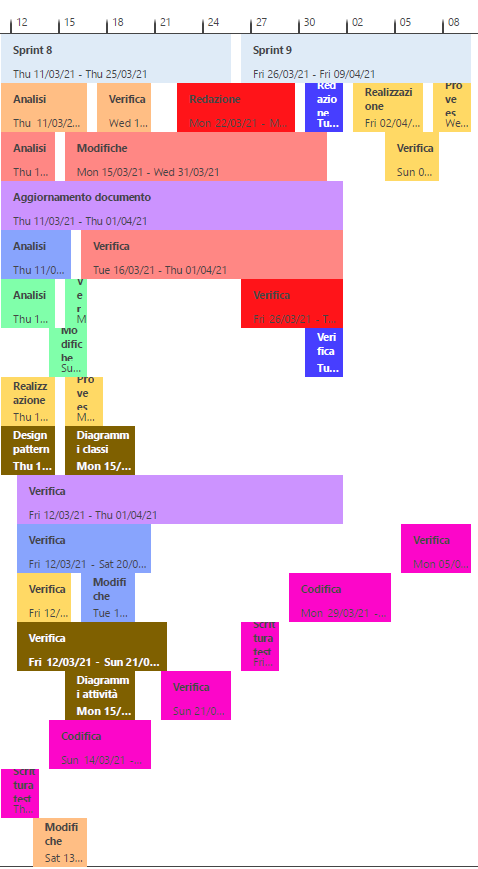
\includegraphics[scale = 0.5]{components/img/sprint8-9.png}
    \caption{Timeline degli sprint che comprendono la  fase di dettaglio e codifica}
    \label{fig:Timeline,sprint 8 e 9, fase di dettaglio e codifica}
\end{figure}

\newpage
\subsection{Validazione e collaudo}
Questo periodo ha inizio il 2021-04-10 e si conclude il 2021-05-09, include lo sprint 8 e lo sprint 9.
Le precondizioni sono:
\begin{itemize}
	\item superamento del colloquio per la Product Baseline;
	\item aggiornamento e correzione dei documenti;
	\item raggiungimento di un prodotto completo, funzionante e di qualità.
\end{itemize}
Le post condizioni sono:
\begin{itemize}
	\item aggiornamento e correzione dei documenti;
	\item esecuzione dei \glo{test} di \glo{sistema} e di accettazione;
	\item consegna dei documenti richiesti alla Revisione di Accettazione.
\end{itemize}
\subsubsection{Attività}
Le attività che vengono svolte sono:
\begin{itemize}
	\item \textbf{Analisi modifiche e \ignore{verifica}:} vengono migliorati e aggiornati i documenti già prodotti (\PdP{}, \G{}, \PdQ{}, \textit{Technology Baseline}, \textit{Product Baseline},\textit{Manuale Utente}, \textit{Manuale Sviluppatore});
	\item \textbf{Sviluppo \ignore{software}:} questa attività consiste nella scrittura dei \glo{test}, nella scrittura del codice e della sua \glo{verifica};
	\item \textbf{\glo{Validazione} e collaudo:} vengono eseguite ulteriori \glo{test} sul prodotto, in modo da garantire la correttezza e un buon livello di qualità;
\end{itemize}
\subsubsection{Diagramma di Gantt, validazione e collaudo}
\begin{figure}[H]
    \centering
    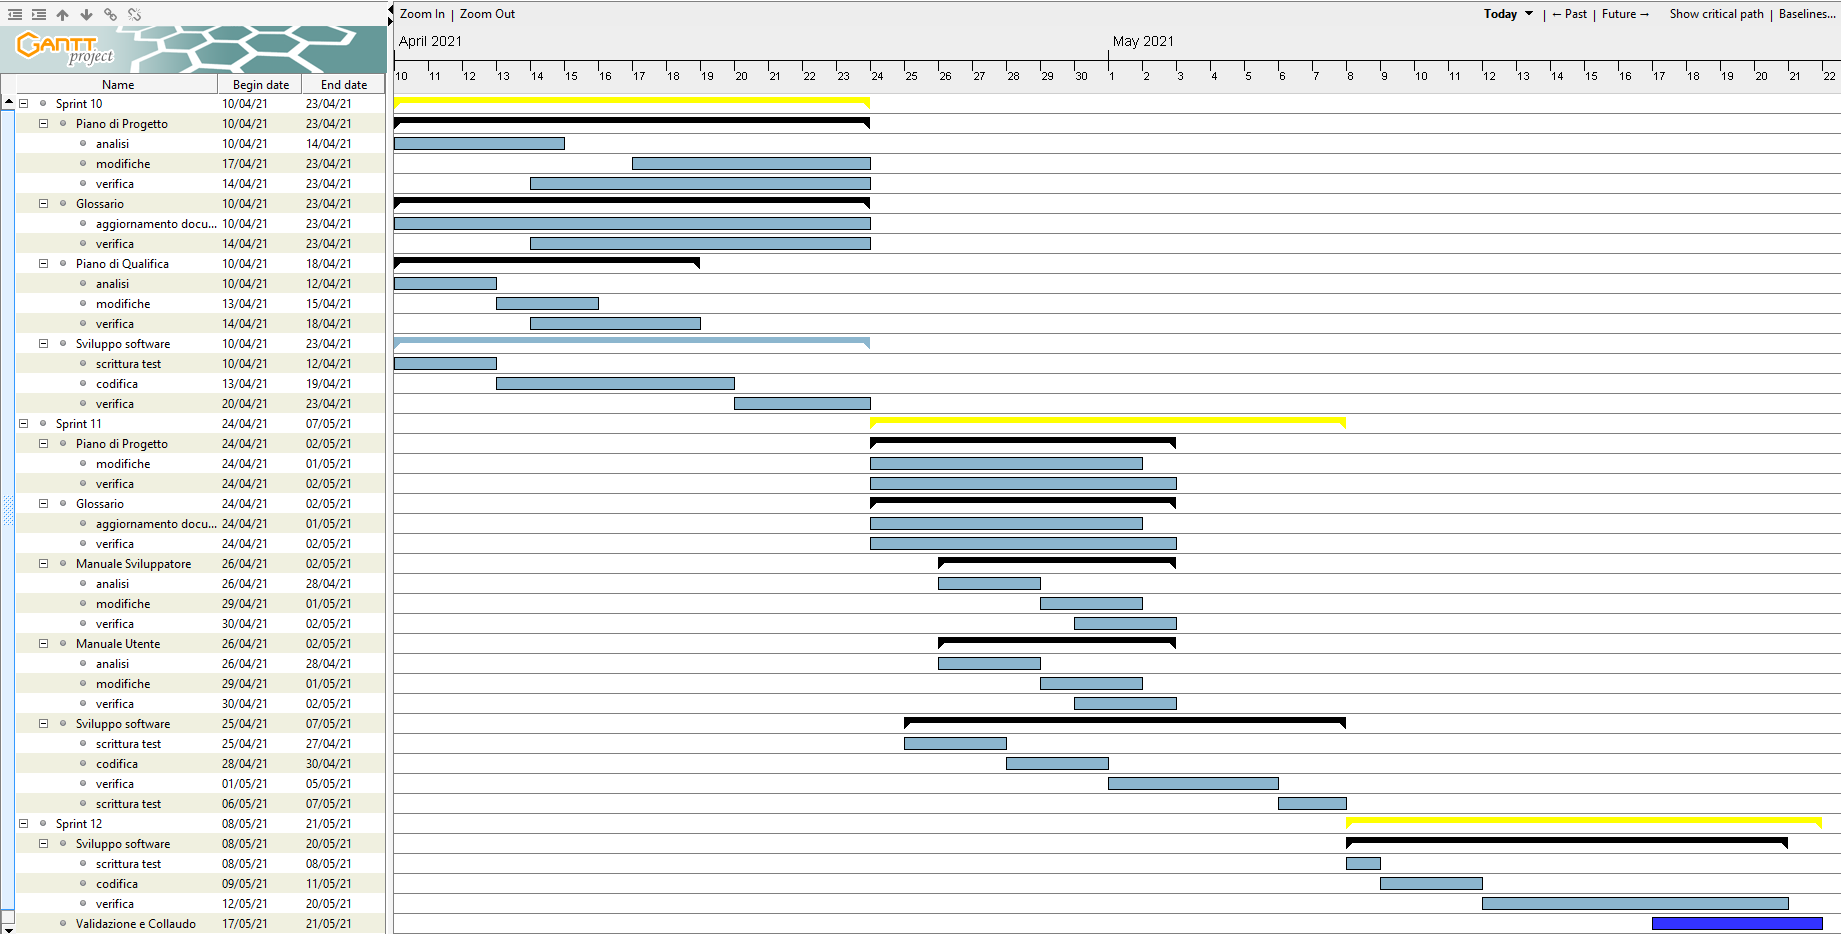
\includegraphics[scale = 0.25]{components/img/validazione_collaudo.png}
    \caption{Diagramma di Gantt della fase di Progettazione di Validazione e Collaudo}
    \label{fig:Diagramma di Gantt, fase di validazione e collaudo}
\end{figure}
\subsubsection{Sprint 10}
Questo sprint ha inizio in data 2021-04-10 e si conclude in data 2021-04-24. Le sue precondizioni sono il raggiungimento degli obiettivi dello sprint precedente.\newline{}
Gli obiettivi da raggiungere durante questo periodo sono:
\begin{itemize}
	\item Aggiornamento, correzione e verifica del \PdP{};
	\item Aggiornamento, correzione e verifica del \PdQ{};
	\item Rifattorizzazione del codice conseguente alla \PB{};
	\item Stesura test;
	\item Implementazione strategia manuale;
	\item Verifica codice;
	\item Aggiornamento del \G{};
	\item Verifica del \G{}.
\end{itemize}
\subsubsection{Sprint 11}
Questo sprint ha inizio in data 2021-04-25 e si conclude in data 2021-05-09. Le sue precondizioni sono il raggiungimento degli obiettivi dello sprint precedente.\newline{}
Gli obiettivi da raggiungere durante questo periodo sono:
\begin{itemize}
	\item Aggiornamento, correzione e verifica del \PdP{};
	\item Aggiornamento, correzione e verifica del \MS{};
	\item Aggiornamento, correzione e verifica del \MU{};
	\item Stesura test;
	\item Implementazione politica manuale nel programma;
	\item Verifica codice;
	\item Aggiornamento del \G{};
	\item Verifica del \G{}.
\end{itemize}
\subsubsection{Timeline: sprint 10 e 11}
\begin{figure}[H]
    \centering
    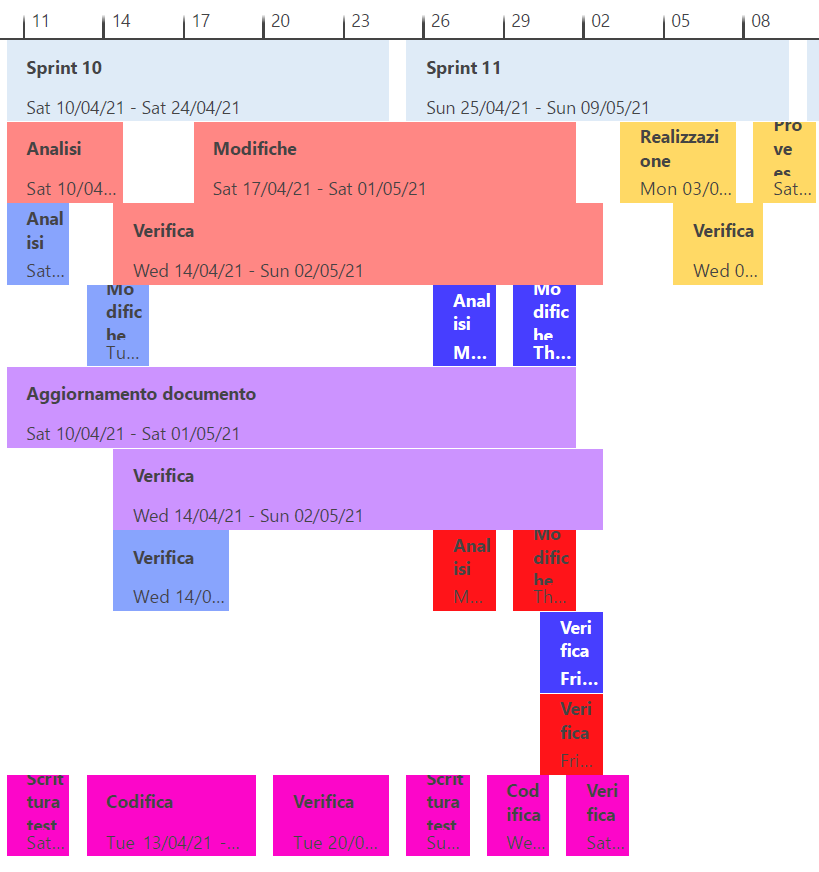
\includegraphics[scale = 0.5]{components/img/sprint10-11.png}
    \caption{Timeline degli sprint che comprendono la  fase di validazione e collaudo}
    \label{fig:Timeline,sprint 10 e 11, fase di validazione e collaudo}
\end{figure}